\subsection{Replikasi basis data}

Replikasi berarti menyimpan salinan data yang sama pada beberapa mesin yang berbeda dan terhubung melalui jaringan \parencite{dataIntensiveApplications}. Terdapat beberapa alasan mengapa hal ini lazim dilakukan, yaitu:

\begin{enumerate}
    \item Untuk menjaga data tetap dekat secara geografis kepada pengguna, sehingga latensi berkurang.
    \item Agar sistem dapat terus berjalan meski terjadi kegagalan pada sebagian sistem, sehingga \textit{availability} meningkat.
    \item Untuk melakukan \textit{scale out} banyaknya mesin yang bisa melayani \textit{read queries}, sehingga meningkatkan \textit{read throughput}.
\end{enumerate}

Salah satu pendekatan yang umum diimplementasikan pada basis data relasional seperti PostgreSQL adalah replikasi berbasiskan \textit{leader and follower}. Satu \textit{node} ditugaskan sebagai \textit{leader} yang menerima operasi \textit{read and write}, lalu setiap perubahan yang terjadi akan direplikasi oleh replika (\textit{follower}). Dengan pola seperti ini, umumnya operasi \textit{write} hanya dapat ditangani oleh \textit{leader} dan operasi \textit{read} dapat ditangani oleh semua \textit{node}.

\begin{figure}
    \centering
    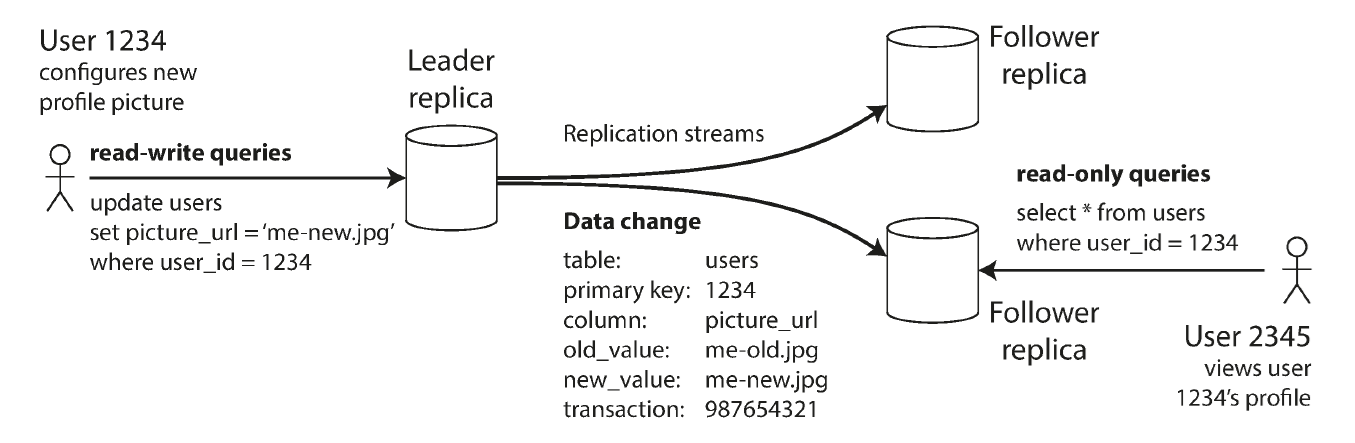
\includegraphics[width=0.8\textwidth]{resources/chapter-2/leader-based-replication.png}
    \caption{\textit{Leader-based (master-slave) replication \parencite{dataIntensiveApplications}}}
    \label{fig:leader-based-replication}
\end{figure}

Selain itu, proses replikasi juga terbagi menjadi dua, yaitu \textit{synchronous replication} dan \textit{asynchronous replication}. Pada \textit{synchronous replication}, data yang akan ditulis juga harus sudah ditulis oleh semua (atau mayoritas) replika sebelum dapat di-\textit{acknowledge}. Pada \textit{asynchronous replication}, data akan ditulis terlebih dahulu pada \textit{leader} lalu perubahannya dipropagasikan kepada \textit{replika}. Setiap pendekatan ini memiliki \textit{tradeoff} tersendiri. \textit{Synchronous replication} menjamin mayoritas \textit{node} memiliki data paling terbaru, tetapi latensi pada proses penulisan akan meningkat, sedangkan pada \textit{asynchronous replication} latensi penulisan jauh lebih kecil, tetapi data pada \textit{replica} menjadi \textit{eventually consistent}. Kedua mode replikasi ini didukung oleh PostgreSQL.